\documentclass{standalone}
\usepackage{PhysicalChemistryNote}
\begin{document}
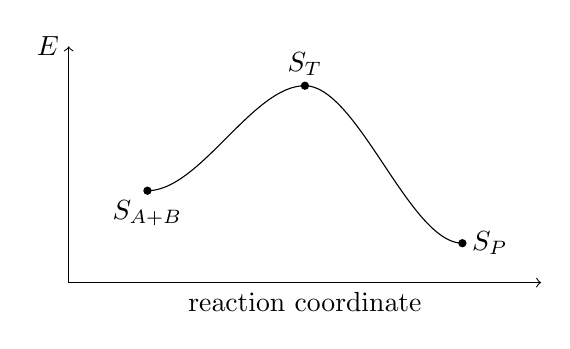
\begin{tikzpicture}
    \draw[->] (0,0)--(6,0) ;
    \node[below] at (3,0) {reaction coordinate};
    \draw[->] (0,0)--(0,3) node[left]{$E$};
    \draw[domain=1:3] plot[smooth] (\x,{(-(\x-2)^3+3*\x-0.5)/3});
    \draw[domain=3:5] plot[smooth] (\x,{((\x-4)^3-3*\x+15)/2});
    \fill (1,7/6) circle (1.5pt) node[below]{$S_{\ce{A}+\ce{B}}$};
    \fill (3,2.5) circle (1.5pt) node[above]{$S_{\ce{T}}$};
    \fill (5,0.5) circle (1.5pt) node[right]{$S_{\ce{P}}$};
    
\end{tikzpicture}
\end{document}